\section{Vision Appendix}
\label{apx:vision}

\begin{figure}[h!]
  \caption{Centroiding being affected by noise}
  \centering
    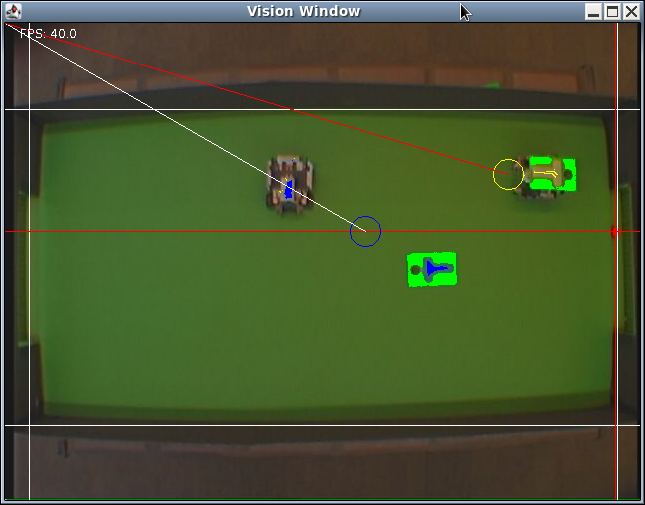
\includegraphics[width=0.5\textwidth]{randy_bins_before.png}
\end{figure}

\begin{figure}[h!]
  \caption{One centroid for each bin, indicated by pink dots}
  \centering
    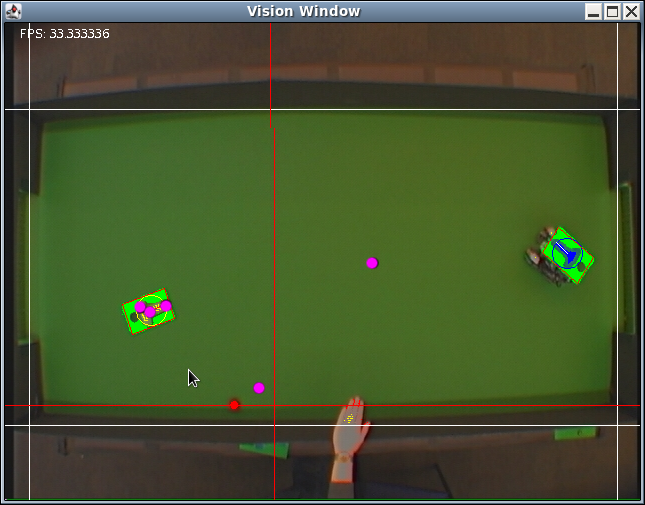
\includegraphics[width=0.5\textwidth]{randy_bins_after_mult.png}
\end{figure}

\begin{figure}[h!]
  \caption{Centroiding being unaffected by noise}
  \centering
    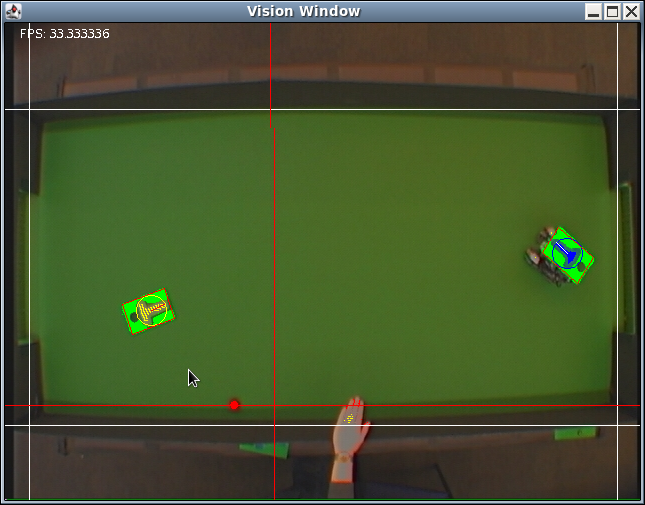
\includegraphics[width=0.5\textwidth]{randy_bins_after.png}
\end{figure}

\begin{figure}[h!]
  \caption{RGB Colour space}
  \centering
    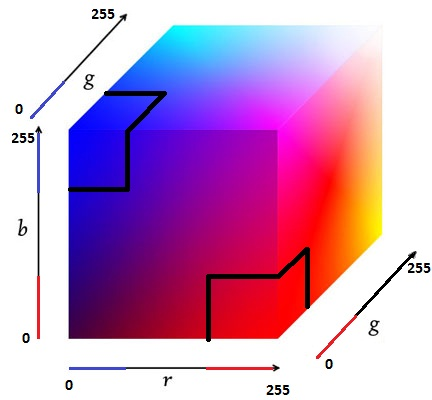
\includegraphics[width=0.5\textwidth]{RGB_Space.jpg}
\end{figure}



%The label is so it can be dynamically refrenced from else where in the
%document
